%%%%%%%%%%%%%%%%%%%%%%%%%%%%%%%%%%%%%%%%%%%%%%%%%%%%%%%%%%%%%%%%%%%%%%%%%%
%% CV-SerafinVelezVarrera 0.1, 2014-10-17				%%
%% Written by Serafín Vélez Barrera <serafa12000@gmail.com> 		%%
%% ---------------------------------------------------------- 		%%
%% Licensed under							%%
%% 	Creative Commons Attribution-NonCommercial-ShareAlike 3.0	%%
%% http://creativecommons.org/licenses/by-nc-sa/3.0/			%%
%%%%%%%%%%%%%%%%%%%%%%%%%%%%%%%%%%%%%%%%%%%%%%%%%%%%%%%%%%%%%%%%%%%%%%%%%%

%%%%%%%%%%%%%%%%%%%%%%%%%%%%%%%%%%%%%%%%%%%%%%%%%%%%%%%%%%%%%%%%%%%%%%%%%%
%				Preámbulo				 %
%%%%%%%%%%%%%%%%%%%%%%%%%%%%%%%%%%%%%%%%%%%%%%%%%%%%%%%%%%%%%%%%%%%%%%%%%%


% Definición del documento
\documentclass{beamer}
\usepackage[utf8x]{inputenc}
\usepackage[spanish]{babel}
\usepackage{beamerthemeshadow}
\usetheme{Antibes}

%Preámbulo -> Definición del título del documento, autor, institución, fecha y fondo para las transparencias.
\title{El Software Libre}
\subtitle{La filosof\'ia convertida en realidad}
\author[Seraf\'in V\'elez Barrera]{Seraf\'in V\'elez Barrera\\ \scriptsize{\texttt{seravb@correo.ugr.es}}}
\date{\today}
\institute{
\includegraphics[scale=0.5]{logo.png}}
\usebackgroundtemplate{
\includegraphics[width=\textwidth]{MarcaDeAgua.png}}


%Documento
\begin{document}
	\begin{frame}
		\titlepage
	\end{frame}


	\begin{frame}
	        \frametitle{Índice}
	        \tableofcontents
	\end{frame}


	\section{¿Qué es el Software Libre?}
		\begin{frame}
			\frametitle{¿Qué es el Software Libre?}
			El Software Libre en sí es una filosofía, pero es incluso más que eso por que se estudia y aplica sobre una gran
			variedad de temas tales como:
			\begin{itemize}
				\item \emph{El Ser Humano}
				\item \emph{La sociedad}
				\item \emph{La moral}
				\item \emph{El conocimiento}
				\item \emph{La libertad}
			\end{itemize}
		\end{frame}
		\begin{frame}
			\frametitle{Importancia}
			\begin{center}
				\Large{¿Debe importarme el Software Libre?}
				\\
				\pause
				\textbf{\huge{SI}}
			\end{center}
			Motivos:
			\begin{itemize}
				\item No vulnera la integridad de las personas.
				\item Transmite confianza y claridad.
				\item Su aplicación nos conlleva a un mundo mejor.
				\item Está respaldado por una gran comunidad de personas.
			\end{itemize}
			\pause
			Y al conseguir que el software sea libre, conseguimos que el conocimiento
			sea libre beneficiándonos todos.
		\end{frame}


	\section{Breve historia}
		\begin{frame}
			\frametitle{Breve historia}
			\begin{itemize}
				\item<1->[70's] El negocio estaba en el hardware y el software era un añadido que en aquellos años se poseía el código fuente
					cambiando notablemente.
				\item<2->[80's] El negocio pasa del harware al software, se crean licencias privativas lo que conlleva a su no divulgación. Así
					Richard M. Stallman crea la FSF (Free Sofware Foundation) en contra de esta pérdida de libertad y crea el proyecto GNU (GNU is 
					Not UNIX) proyecto para crear un Sistema Operativo Libre
				\item<3->[90's] Linus Torvalds crea el núcleo de Linux que junto con el proyecto GNU se crea un Sistema Operativo totalmente libre.
				\item<4->['00-Hoy] Ya el Software Libre se ha hecho un gran hueco en la sociedad si lo medimos a la influencia que tenía en sus comienzos.
			\end{itemize}
		\end{frame}


	\section{Aclaraciones y Mitos}
		\begin{frame}
			\frametitle{Aclaraciones}
			\begin{columns}
				\begin{column}[l]{5cm}
					\begin{itemize}
						\item<2-> Software Libre = Gratis
						\item<3-> Licencia = Propietario
						\item<4-> Límites de libertades
						\item<5-> Licencias+Construcción
						\item<6-> Licencias+Ejecución
					\end{itemize}
				\end{column}
				\begin{column}[r]{5cm}
					\begin{itemize}
						\item<2-> FALSO
						\item<3-> FALSO (sólo derechos)
						\item<4-> Cada vez más complicado
						\item<5-> ¿Herramienta libre?
						\item<6-> ¿Ejecución libre?
					\end{itemize}
				\end{column}
			\end{columns}
		\end{frame}
		\begin{frame}
			\frametitle{Mitos sobre el Software Libre}
			\begin{itemize}
				\item<2-> El Software Libre es sólo ``Linux''
				\item<3-> Software Libre es aquel que solo funciona en ``Linux''
				\item<4-> El Software Privativo es más seguro.
				\item<5-> El Software Libre es difícil de usar.
			\end{itemize}
		\end{frame}


	\section{Clasificación gráfica}
		\begin{frame}\frametitle{Clasificación}
			\includegraphics[width=\textwidth, keepaspectratio=true]{Clasificacion0.png}
		\end{frame}
		\begin{frame}\frametitle{Clasificación}
			\includegraphics[width=\textwidth, keepaspectratio=true]{Clasificacion1.png}
		\end{frame}
		\begin{frame}\frametitle{Clasificación}
			\includegraphics[width=\textwidth, keepaspectratio=true]{Clasificacion2.png}
		\end{frame}
		\begin{frame}\frametitle{Clasificación}
			\includegraphics[width=\textwidth, keepaspectratio=true]{Clasificacion3.png}
		\end{frame}
		\begin{frame}\frametitle{Clasificación}
			\includegraphics[width=\textwidth, keepaspectratio=true]{Clasificacion4.png}
		\end{frame}


	\section{¿Dónde se usa?}
		\begin{frame}
			\frametitle{¿Dónde se usa?}
			Hay multitud de ejemplos donde está el Software Libre, por ejemplo tenemos los siguientes:
			\begin{itemize}
				\item<2-> Servidores de internet
				\item<3-> Routers
				\item<4-> Electrodomésticos.
				\item<5-> Domótica/Robótica.
			\end{itemize}
		\end{frame}


	\section{Conceptos}
		\begin{frame}
			\frametitle{Modelo de negocio}
			\includegraphics[width=\textwidth, keepaspectratio=true]{herramientas_productos_servicios1.png}
			\pause
			\begin{itemize}
				\item Desarrollo
				\item Corrección de errores
				\item Traducción
				\item Instalación
				\item Configuración
			\end{itemize}
		\end{frame}
		\begin{frame}
			\frametitle{Modelo de negocio}
			\includegraphics[width=\textwidth, keepaspectratio=true]{herramientas_productos_servicios2.png}
			\pause
			\begin{itemize}
				\item Soporte
				\item Formación
				\item Mejoras
				\item Infraestructuras
				\item Adaptación
			\end{itemize}
		\end{frame}
		\begin{frame}
			\frametitle{Ventajas frente a inconvenientes}
			\begin{columns}
				\begin{column}[l]{5cm}
					\begin{center}
						VENTAJAS
					\end{center}
					\begin{itemize}
						\item<2-> Usuario/Cliente no cautivos
						\item<3-> Reutilización
						\item<4-> Seguridad
						\item<5-> Oportunidad de negocio
						\item<6-> Se eliminan los monopolios
						\item<7-> Legal
					\end{itemize}
				\end{column}
				\begin{column}[r]{5cm}
					\begin{center}
						INCONVENIENTES
					\end{center}
					\begin{itemize}
						\item<2-> Usuarios/Clientes rehacios al cambio
						\item<3-> La sociedad no lo conoce bien
						\item<4-> En ocasiones falta de publicidad y/o marketing
						\item<5-> Posibilidad en que no existan algunas herramientas específicas
						\item<6-> Cualificación del profesional administrador
					\end{itemize}
				\end{column}
			\end{columns}
		\end{frame}
		\begin{frame}
			\frametitle{Esto me gusta pero me da miedo}
			\begin{enumerate}
				\item Haces muy bien si te gusta.
				\item Si no es así por que piensas que es un utopía, debo decirte que no es así.
			\end{enumerate}
			Si te da miedo el cambio no temas, por que con el Software Libre no se cumple el dicho de:\\
			\begin{center}
				\textbf{\emph{Más vale lo malo conocido que lo bueno por conocer}}
			\end{center}
			\pause
			El Software Libre convence, no vence;\\
			\pause
			No se impone, se expone;\\
			\pause
			Más que un producto, es una forma de hacer;\\
			\pause
			Ni es pirata, ni es gratis.\\
			\textit{Tweet de: \@ tavi\_8}
		\end{frame}


	\section{Conclusiones}
		\begin{frame}
			\frametitle{Lo que hemos visto}
			Hemos visto cuáles son las ideas en las que se basa el Software Libre para nacer, crearse y mantenerse como parte de la vida y sociedad
			que nos rodea.
			\\
			Siendo posible un modelo de negocio para empresas y donde se han creado (y lo seguirán haciendo) grandes nichos de mercado y grandes ideas.
		\end{frame}
		\begin{frame}
			\frametitle{Conclusión}
			El Software Libre representa el futuro que lo veremos implantado en gran parte de la sociedad cuando gran parte de esta cambie 
			su forma de pensar y vea que este tipo de software no es perjudicial y que no sólo unos ``eruditos'' son capaces de crear, mantener,
			difundir, etc.
		\end{frame}
		\begin{frame}
			\begin{center}
				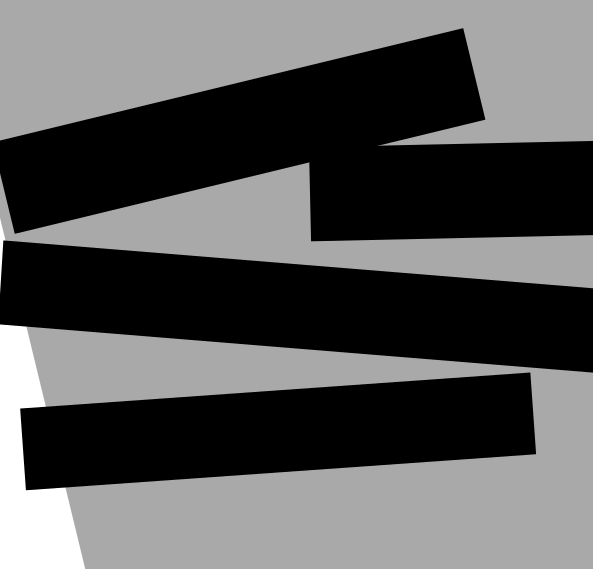
\includegraphics[height=\textheight, keepaspectratio=true]{preguntas_dudas_aclaraciones.png}
			\end{center}
		\end{frame}
		\begin{frame}
			\begin{center}
				\Huge{\textbf{MUCHAS GRACIAS}}
			\end{center}
		\end{frame}


	\begin{frame}
		\frametitle{Fuentes}
		\begin{itemize}
			\item http://fsf.org
			\item http://osl.ugr.es
			\item http://es.wikipedia.org/wiki/GNU/Linux
		\end{itemize}
	\end{frame}


	\begin{frame}
		\frametitle{Distribuciones de GNU/Linux}
		\begin{itemize}
			\item http://www.ubuntu.com/
			\item http://www.debian.org/index.es.html
			\item http://fedoraproject.org/es/
			\item http://www.linuxmint.com/
			\item http://www.redhat.com/
			\item http://www.guadalinex.org/
		\end{itemize}
	\end{frame}


	\begin{frame}
		\frametitle{Licencia}
		\begin{figure}
			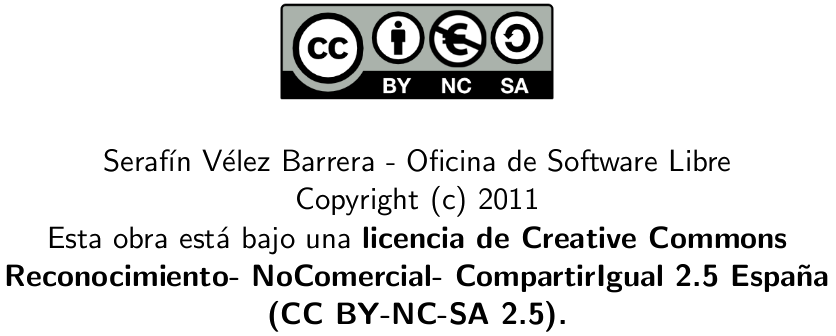
\includegraphics[width=\textwidth, height=\textheight, keepaspectratio=true]{./Licencia/LicenciaCC_Autor.png}
		\end{figure}
	\end{frame}
\end{document}
